\section{Analisi dei rischi}

	Di seguito verranno definiti i rischi individuati dal gruppo Dream Corp. associando ad ognuno di essi un impatto sul progetto e una probabilità che si verifichi. Viene associato inoltre una risposta contenitiva del rischio. 
	\begin{table}[!htpb]
		\centering
		\renewcommand{\arraystretch}{2} 
		\rowcolors{2}{gray!25}{white}
		\begin{tabular}{|c|p{3.6cm}|c|c|p{3.6cm}|}
			\rowcolor{orange!50}
			\hline
			\textbf{Identificativo} & \textbf{Descrizione rischio} & \textbf{Probabilità} & \textbf{Impatto} & \textbf{Risposta Contenitiva}\\
			\hline
			R1 & Errata stima della durata delle attività da programmare & Alta & Alto & Considerare sempre un certo slack temporale e pianificazione all’indietro\\
			\hline
			R2 & Conflitti interni al gruppo di progetto & Bassa & Basso & Team building sociale e confronti diretti\\
			\hline
			R3 & Sottostima del tempo richiesto per l’apprendimento di nuove tecnologie (GitHub, Grafana,...) & Media & Medio & Confronto con esperti per dubbi e chiarimenti al fine di prevenire ritardi\\
			\hline
			R4 & Problemi Software di terze parti (perdita di dati su GitHub) & Molto  Bassa & Basso &  Backup due volte la settimana\\
			\hline
			R5 & Ridefinizione dei requisiti & Bassa & Molto Alto & Ritorno alla fase di analisi\\
			\hline
		\end{tabular}
		\caption{Analisi dei Rischi}
	\end{table}
	\clearpage
	Per analizzare l'impatto che un rischio puó avere sul progetto adottiamo una scala numerica così definita:
	\begin{itemize}
		\item Molto Basso: 1
		\item Basso: 2
		\item Medio: 3
		\item Alto: 4
		\item Molto Alto: 5
	\end{itemize}
	Ed inoltre creiamo una scala di probabilità discreta così definita:
	\begin{itemize}
		\item Molto Bassa: 10\%
		\item Bassa: 25\%
		\item Media: 50\%
		\item Alta: 75\%
		\item Molto Alta: 90\%
	\end{itemize}
	L’utilizzo di una scala numerica ci permette di analizzare più efficacemente l’impatto probabile all’interno del nostro progetto e quindi anche di pianificare all’indietro tenendo conto di queste analisi. \\ \\ Procederemo adesso con il calcolo della \textit{magnitudo} di ogni rischio.
	La magnitudo viene calcolata come prodotto dell'impatto del rischio e la probabilità che esso si verifichi. \\ \\
	Magnitudo = Impatto * Probabilità \\ \\
	\begin{table}[!htpb]
		\centering
		\renewcommand{\arraystretch}{2} 
		\rowcolors{1}{white}{gray!25}
		\begin{tabular}{|c|c|c|c|}
		    \rowcolor{orange!50}
		    \hline
		    \textbf{Identificativo} & \textbf{Probabilità} & \textbf{Impatto} & \textbf{Magnitudo}\\
			\hline
			R1 & 75\% & 4 & 3 \\
			\hline
			R2 &  25\%  & 2  & 0.5 \\
			\hline
			R3  & 50\%  & 3  & 1.5 \\
			\hline
			R4  & 10\% &  2 &  0.2 \\
			\hline
			R5  & 25\%  & 5  & 1.25 \\
			\hline
			\textbf{Media}  & \textbf{37 \%}&  \textbf{3.2} &  \textbf{1,29}\\
			\hline
		\end{tabular}
		\caption{Probabilità dei Rischi}
	\end{table}
	\newline
	\begin{figure}
	    \centering
	    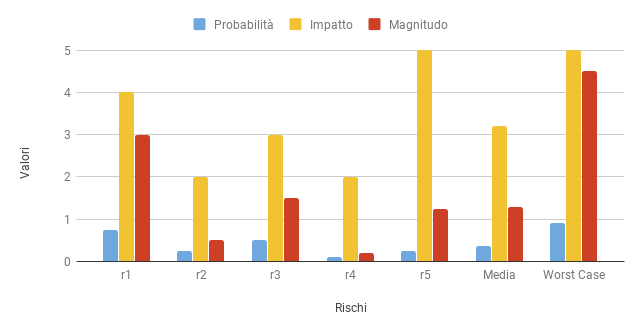
\includegraphics[scale=0.6]{elaborazione_manitudo.png} 
	    \caption{Grafico Confronto Probabilità-Impatto-Magnitudo}
	\end{figure}
	\newline
	Dall'elaborazione presenta nella tabella 8 otteniamo:
	\begin{itemize}
	    \item Probabilità media di un rischio = 37 \% (Bassa-Media);
	    \item Impatto medio di un rischio = 3.2 (Medio);
	    \item  Magnitudo media = 1,29.
	\end{itemize}
	Magnitudo nel caso pessimo: 5 (impatto massimo) * 90 \%(probabilità molto alta) = 4,5.\\
	Predisposizione al rischio, calcolata come rapporto tra magnitudo media e magnitudo nel caso pessimo = 1,29/4,5 = \textbf{ 28,7 \% }\\ \\
	Concludendo possiamo ritenere la nostra predisposizione al rischio abbastanza bassa.
